\chapter{Практические задания}

\section*{Задание 1. Напишите функцию, которая уменьшает на 10 все числа из списка-аргумента этой функции, проходя по верхнему уровню списковых ячеек. ( * Список смешанный структурированный)}

\begin{lstinputlisting}[
	caption={Задание 1, mapcar},
	label={lst:t1-1},
	style={lsp},
	linerange={1-7},
	]{../src/main.lsp}
\end{lstinputlisting}

\begin{lstinputlisting}[
	caption={Задание 1, mapcan},
	label={lst:t1-2},
	style={lsp},
	linerange={10-18},
	]{../src/main.lsp}
\end{lstinputlisting}

\section*{Задание 2. Написать функцию которая получает как аргумент список чисел, а возвращает список квадратов этих чисел в том же порядке.}

\begin{lstinputlisting}[
	caption={Задание 2, mapcar},
	label={lst:t2-1},
	style={lsp},
	linerange={20-24},
	]{../src/main.lsp}
\end{lstinputlisting}

\begin{lstinputlisting}[
	caption={Задание 2, mapcan},
	label={lst:t2-2},
	style={lsp},
	linerange={26-30},
	]{../src/main.lsp}
\end{lstinputlisting}

\section*{Задание 3.  Напишите функцию, которая умножает на заданное число-аргумент все числа из заданного списка-аргумента, когда}
a) все элементы списка --- числа,

б) элементы списка -- любые объекты.

\begin{lstinputlisting}[
	caption={Задание 3, a, mapcar, mapcon},
	label={lst:t3-1},
	style={lsp},
	linerange={32-42},
	]{../src/main.lsp}
\end{lstinputlisting}

\clearpage

\begin{lstinputlisting}[
	caption={Задание 3, b, mapcar, mapcon},
	label={lst:t3-2},
	style={lsp},
	linerange={44-60},
	]{../src/main.lsp}
\end{lstinputlisting}


\section*{Задание 4. Написать функцию, которая по своему списку-аргументу lst определяет является ли он палиндромом (то есть равны ли lst и (reverse lst)), для одноуровнего смешанного списка. }


\begin{lstinputlisting}[
	caption={Задание 4},
	label={lst:t4},
	style={lsp},
	linerange={62-71},
	]{../src/main.lsp}
\end{lstinputlisting}

\section*{Задание 5. Используя функционалы, написать предикат set-equal, который возвращает t, если два его множества-аргумента (одноуровневые списки) содержат одни и те же элементы, порядок которых не имеет значения.}

\begin{lstinputlisting}[
	caption={Задание 5},
	label={lst:t5},
	style={lsp},
	linerange={73-81},
	]{../src/main.lsp}
\end{lstinputlisting}

\section*{Задание 6. }
Напишите функцию, select-between, которая из списка-аргумента, содержащего только
числа, выбирает только те, которые расположены между двумя указанными числами - 
границами-аргументами и возвращает их в виде списка (упорядоченного по 
возрастанию  (+ 2 балла))	

\begin{lstinputlisting}[
	caption={Задание 6},
	label={lst:t6},
	style={lsp},
	linerange={83-93},
	]{../src/main.lsp}
\end{lstinputlisting}

\section*{Задание 7. Написать функцию, вычисляющую декартово произведение двух своих списков-аргументов.}

\begin{lstinputlisting}[
	caption={Задание 7},
	label={lst:t7},
	style={lsp},
	linerange={95-99},
	]{../src/main.lsp}
\end{lstinputlisting}

\section*{Задание 8. Почему так реализовано reduce, в чем причина?}

\begin{lstinputlisting}[
	caption={Задание 8},
	label={lst:t8},
	style={lsp},
	linerange={101-102},
	]{../src/main.lsp}
\end{lstinputlisting}

Если список пуст, а начальное значение не задано, то вызывается функция без аргументов, а reduce возвращает то, что вернёт функция. Функция сложения без аргументов возвращает 0, а функция умножения возвращает 1.

\section*{Задание 9. }
Пусть list-of-list список, состоящий из списков. Написать функцию, которая вычисляет сумму длин всех элементов list-of-list (количество атомов), т.е. например для аргумента ((1 2) (3 4)) -> 4.

\clearpage

\begin{lstinputlisting}[
	caption={Задание 9},
	label={lst:t9-1},
	style={lsp},
	linerange={104-112},
	]{../src/main.lsp}
\end{lstinputlisting}


%\begin{figure}[h!]
%	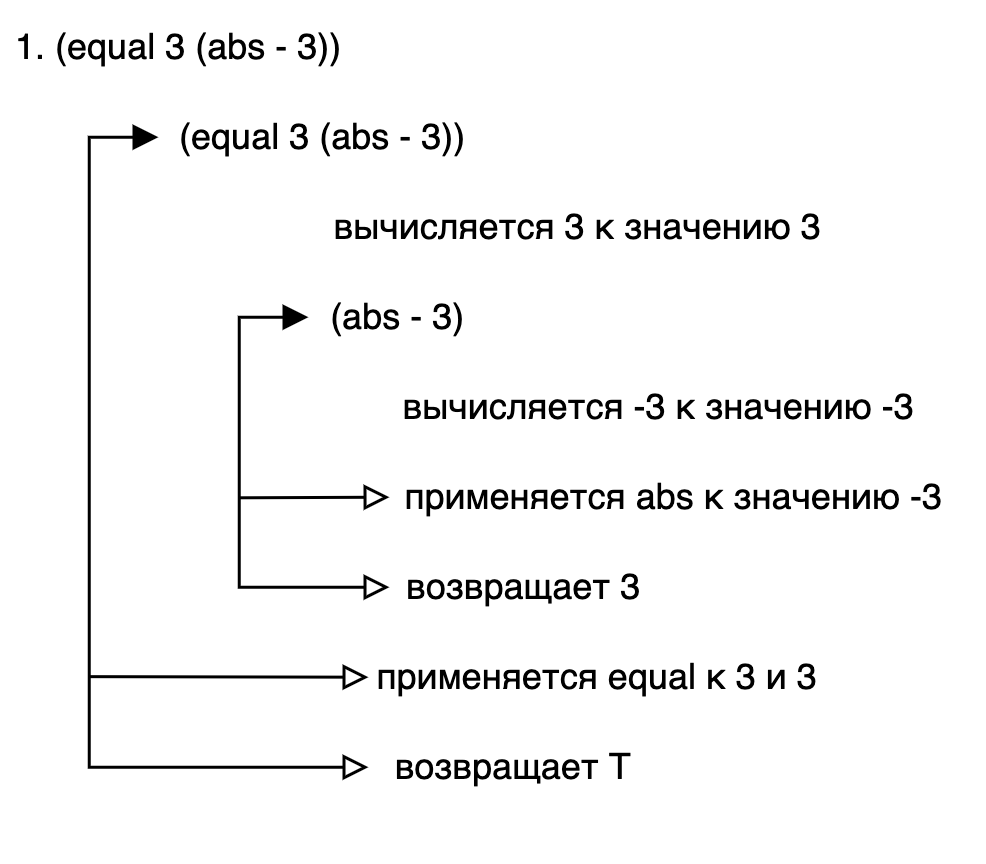
\includegraphics[scale=0.6,left]{task1.1}
%\end{figure}



